
%(BEGIN_QUESTION)
% Copyright 2015, Tony R. Kuphaldt, released under the Creative Commons Attribution License (v 1.0)
% This means you may do almost anything with this work of mine, so long as you give me proper credit

Have some fun writing simple ``exploratory'' or ``demonstration'' ladder-diagram PLC programs to perform different functions.  Feel free to explore the following instruction types:

\begin{itemize}
\item{} Contacts and coils
\item{} Counters (up, down, up/down)
\item{} Timers (on-delay, off-delay, retentive)
\item{} Sequencing instructions
\item{} Math instructions (add, subtract, multiply, divide)
\end{itemize}

Identify some realistic applications for PLC programs using counters and timers.  What sorts of real-life processes might benefit from a PLC function where something turns on or off after a definite number of counts applied to the PLC input, or after a certain amount of time has passed?

\vskip 10pt

{\bf Note: this simple exercise may seem trivial, but it holds the key to self-instruction on PLC programming!}  Having your very own PLC to work with in the classroom is a tremendously powerful learning tool.  Whenever you encounter a new programming instruction (e.g. a timer, a math instruction, etc.) that you do not yet know how to use, you may explore that instruction's properties and behavior by creating a simple program in your PLC with nothing but that instruction.  Your PLC's {\it User Manual} or {\it Instruction Set} reference manual will show you the basic syntax of the instruction, which you may copy verbatim as an example.  Once this simple program is loaded into your PLC's memory, you can ``play'' with it to see its live behavior while viewing the program online.

Once you have directly observed how the instruction works, your next step is to add comments to the program describing how that instruction works in your own words.  Be as detailed as possible here, treating this activity as though you were asked to explain everything to someone who knew absolutely nothing about the instruction.  These comments will serve as notes to yourself later, when you need to refresh your memory on how a particular instruction functions or what it is used for.

\vskip 10pt

{\it Do not be surprised if your instructor asks you to show your demonstration program(s) for particular instructions in the future!  If you experience difficulty using a particular instruction in a programming assignment, your instructor may check to see if you have created and run a demonstration program to learn how that instruction is supposed to function.}

\vskip 10pt

Refer to the ``Answer'' section of this question to see some examples of what such a demonstration program might look like.

\vskip 20pt \vbox{\hrule \hbox{\strut \vrule{} {\bf Suggestions for Socratic discussion} \vrule} \hrule}

\begin{itemize}
\item{} A helpful tip when writing your own demonstration programs is to save each one with a filename that makes it easy to locate on your personal computer.  For example, you might wish to name each of your demonstration programs beginning with the word ``Demo'' and using underscore characters to separate descriptive words (or instruction names) in the rest of the filename.  Some examples are shown here:
\itemitem{} {\tt Demo\_contacts\_coils}
\itemitem{} {\tt Demo\_upcounter}
\itemitem{} {\tt Demo\_downcounter}
\itemitem{} {\tt Demo\_TOF\_timer}
\itemitem{} {\tt Demo\_TON\_timer}
\itemitem{} {\tt Demo\_ADD\_instruction}
\end{itemize}

\underbar{file i00120}
%(END_QUESTION)





%(BEGIN_ANSWER)

\noindent
{\bf Demonstration program showing some basic bit instructions in an Allen-Bradley MicroLogix PLC:}

$$\includegraphics[width=15.5cm]{i00120x01.eps}$$


\filbreak

\noindent
{\bf Demonstration program showing ``up'' and ``down'' counter instructions in an Allen-Bradley MicroLogix PLC:}

$$\includegraphics[width=15.5cm]{i00120x03.eps}$$


\filbreak

\noindent
{\bf Demonstration program showing an on-delay timer instruction in an Allen-Bradley MicroLogix PLC:}

$$\includegraphics[width=15.5cm]{i00120x02.eps}$$

%(END_ANSWER)





%(BEGIN_NOTES)

\vfil \eject

\noindent
{\bf Summary Quiz:}

This exercise makes an excellent summary quiz: having the student show at least one of their new demonstration programs, fully commented and operating.  Encourage them to be verbose in their comments, making the rung comments so clear and illustrative that anyone reading it will be able to learn how that instruction functions.  {\it Ask them to literally demonstrate what they have learned about the various instructions by running their programs and narrating what they see the instructions doing when viewed online (with status coloring and numerical values shown live).}

\vskip 10pt

{\it Remind students that you (as the instructor) will have them refer to their demonstration programs if they ever encounter trouble using a particular instruction in the future.  The point of doing this is to instill the good habit of writing demonstration programs for self-directed PLC learning as well as ensure that their demonstration programs are documented completely enough to be useful in addressing future questions and problems they may have.}

\vskip 10pt

In my experience as a teacher, most students strongly resist writing demontration programs, thinking such exercises are a waste of time, and that they will learn better by having someone simply tell them how a particular PLC instruction functions.  What actually happens if an instructor directly tells a student how to use an instruction, however, is that the student(s) almost always return to the instructor asking for the same help again in the future (because they didn't really learn the last time).  When students have learned to write their own demonstration programs, they have learned how to teach themselves PLC programming, which is a far more valuable and longer-lasting acquisition than any targeted programming help you as their instructor could possibly dispense to them.



%INDEX% PLC, exploratory question (ladder logic programming with counters and timers)

%(END_NOTES)


